\documentclass{article}
\usepackage[flushleft]{threeparttable}
\usepackage{rotating}
\usepackage{tablefootnote}
\usepackage{tocbibind}
\usepackage{float}
\usepackage{systeme}
\usepackage{amsmath}
\usepackage{mathtools}
\usepackage{natbib}
\usepackage{tikz}
\usepackage{pgfplots}
\usepackage{amsfonts}
\usetikzlibrary{positioning,arrows, calc, arrows, fit, shadows} 
\usepackage{caption}
\captionsetup{justification=raggedright,singlelinecheck=false}
\usepackage{geometry}
\usepackage{setspace}
\usepackage[procnames]{listings}
\pgfplotsset{compat=1.16}
\geometry{
	a4paper,
	left=2cm,
	bottom=2cm,
	right=2cm,
	top=2cm
}
%\setlength{\parindent}{4pt}
\onehalfspacing
\lstset{language=python, basicstyle=\ttfamily\footnotesize}

\begin{document}
	
\section*{1st March}

Machine learning (ML) is the study of computer algorithms that can improve automatically through experience and by the use of data. It is seen as a part of artificial intelligence.
	
\bigskip

Machine learning is the science of getting computers to act without being explicitly programmed. (Arthur Samuel 1959)
	
\bigskip

Machine Learning is concerned with the automatic discovery of regularities in data through the use of computer algorithms and with the use of these regularities to take actions. (Christopher M. Bishop)

\bigskip

The goal of machine learning is to develop methods that can automatically detect patterns in data, and then to use the uncovered patterns to predict future data or other outcomes of interest. (Kevin P. Murphy)

\bigskip


Machine Learning is about predicting the future based on the past (Hal Daume III)


\bigskip

	
The idea behind ML is that we give to th computer data inputs and an output and it will return a program that given data will return the correct output.


\bigskip

ML allows computer to acquire knowledge, which is acquired through algorithms by learning and inferring from data. Knowledge is represented by a model which is used on future data.


\subsection*{When learning from data}
ML is used when human expertise does not exist (navigation on Mars); humans cannot explain their expertise (speech recognition); models must be customized (personalized medicine); model are based on huge amount of data (genomics).

Today the most important when using ML is when we have a huge amount of data and we want to recognize e generate a pattern.


\textbf{Recognizing patterns. }Handwritten digits, facial identities or facial expressions, medical images or data.

\textbf{Generating patterns. } Generating images or motion sequences

\textbf{Recognizing anomalies. } Unusual credit card transactions, unusual patterns of sensor readings, unusual patterns in video surveillance

\textbf{Prediction. } Future stock prices or currency exchanges rates, autonomous driving, predict best moves (go, chess, ...).


\bigskip


\subsection*{ML pipeline}
We start from a training data from which the machine learn and then produces a model. Then given as input testing data, the model produced before is used in order to predict the future

For example, given as input training images of cats and dogs with labels "cat" and "dog", the machine recognize some of the features and it is trained to classify correctly dogs and cats. Then given an image, the machine recognize the features on which it was trained and predict the correct output
	
	
\subsection*{T. Mitchell, 1970}

A computer program is said to learn from experience \emph{E} with respect to some class of tasks \emph{T} and performance measure \emph{P}, if its performance at tasks in \emph{T}, as measured by \emph{P}, improves with experience \emph{E}.

Summing up, ML is the sudy of algorithms that improve their performance \emph{P} at some task \emph{T} with experience \emph{E}. A well defined learning task is given by \(< T, P, E >\).

\subsubsection*{Examples}

\textbf{T} - recognizing handwritten words, \textbf{P} - percentage of words correctly classified, \textbf{E} - database of human labeled images and handwritten words.

\textbf{T} - driving on four lane highways using vision sensors, \textbf{P} - average distance traveled before a human judged error, \textbf{E} - sequence of images and steering commands recorded while observing a human driver.

\textbf{T} - categorize emails as spam or legitimate, \textbf{P} - percentage of emails correctly classified, \textbf{E} - database of emails some with human given labels


\subsection*{Related areas}
Data mining: data analysis, not prediction, though often involves some shared techniques. 

Inference and/or estimation in statistics.

Patter recognition in engineering and signal processing in electrical engineering.

 Optimization.
	

%\includegraphics[keyvals]{imagefile}	
	

\subsection*{ML, AI and DL}

\emph{Artificial Intelligence} is a program that can sense, reason, act and adapt. Inside it we have \emph{Machine Learning} in whihc we have algorithms whose performance improve as they are exposed to more data over time. Finally, inside ML we have \emph{Deep Learning} in which multilayered neural networks learn from vast amount of data.


\subsection*{Deep Learning}

Deep learning allows computational models that are composed of multiple processing layers to learn representations of data with multiple levels of abstraction.

DL means using a neural network with several layers of nodes between input and output. The series of layers between input and output compute relevant features automatically in a series of stages, just as our brains seem to.

It learns the representation of the data during the training process. Models learns alone and finds some patterns/features. The new data constructed by the model in some way regress on the original input.

\bigskip

\textbf{Examples of DL. } Object recognition (2012); object detection; image captioning (2015); image synthesis; speech recognition (2009)

	
\bigskip

Deep learning has seen a revolution recently. That because now we have a huge amount of data, increased computational power. Also, a growing number of ML algorithms and theory developed by researchers and increased support from industry
	
\newpage


\section*{3rd March}

In statistical modeling (programming), we collect data, verify that it is clean (otherwise correct or discard),and then use this clean dataset to test hypotheses and make predictions and forecasts. The aim is to represent complex issues in relatively generalizable terms, which is to say, terms that explain most events studied. Effectively, we program the algorithm to perform certain functions based on the data we submit. The algorithm is static. It needs a programmer to tell it what to do when it is fed with data


In machine learning, rather than pre-selecting a model and feeding data into it, is the data that determines which analytic technique should be selected to best perform a task. The computer uses the data that it has to select and train the algorithm, which is no longer static. It analyses the data to which it is exposed, makes a determination on the best course of action, and then acts. In essence, it “learns” from the data and in doing so, knowledge can be extracted from the data.


In machine learning what we do is: collect (labeled) data, extract features, define a family of models, train (find the model that minimizes the error) and the evaluate the model.

\subsection*{Task}
A task represents the type of prediction being made to solve a problem on some data. We can identify a task with the set of functions that can potentially solve it. In general, it consists of functions assigning each input \(x \in \mathcal{X}\)an output \(y \in \mathcal{Y}\)
\[f: \mathcal{X} \rightarrow \mathcal{Y} \qquad \mathcal{F}_{task} \subset  \mathcal{Y}^{\mathcal{X}}\]

\(\mathcal{X} \) is the input space, \(\mathcal{Y} \) is the output space, and \(\mathcal{F} \) is the task space, the set of all the possible \emph{f}


The nature of \(\mathcal{X}, \mathcal{Y} \text{ and } \mathcal{F}\) depends on the type of problem/application.

	
\subsubsection*{Classification}

Find a function \(f \in \mathcal{Y}^{\mathcal{X}}\) assigning each input \emph{x} a discrete label
\[f(x) \in \mathcal{Y} = \{c_1, c_2, ..., c_k\}\]

where \(c_1, ..., c_k\) are class labels. 
For example, in a binary classification we can assign 1 if the picture has a bird, 0 otherwise.



\subsubsection*{Regression}

Find a function \(f \in \mathcal{Y}^{\mathcal{X}}\) assigning each input \emph{x} a continuous label. For example, in object detection we have to predict coordinates which are a set of numbers.
	
	
\subsubsection*{Density estimation}
Find a probability distribution \( f \in \Delta(\mathcal{X})\) that fits the data \(x \in \mathcal{X}\). In this case there is not a reference to an output space, but we make a reasoning on the input
	

\subsubsection*{Clustering}
Find a function \(f \in \mathbb{N}^{\mathcal{X}}\) that assigns each input \(x \in \mathcal{X}\) a cluster index \(f \in \mathbb{N}\). In this case the algorithms tells us which inputs are similar and  belong to the same group (cluster).
	
	
\subsubsection*{Dimensionality reduction}
Find a function \(f \in \mathcal{Y}^{\mathcal{X}}\) mapping each high dimensional input \emph{x} to a lower dimensional embedding \(f(x) \in \mathcal{Y}\). For example, transform a 3D image in 2D, from rgb to binary



\subsection*{Data}
There are a set of samples, each of which is mapped to a feature (label), e.g. the picture of an apple and the features of colors and shapes.

Each data has a (fixed size) vector of features.

	
\bigskip
Data are in the form of a distribution called \(P_{data}\). In supervised learning (classification and regression) we have \(P_{data} \in \Delta(\mathcal{X} \times \mathcal{Y})\). In unsupervised learning (density estimation, clustering and dimensionality reduction) we have \(P_{data} \in \Delta(\mathcal{X})\)
	
	
	
\bigskip

In supervised and unsupervised the data distribution \(P_{data}\) is typically unknown. What we can do is sampling from the distribution and obtain a set of data \(D_n\)


\subsection*{Train, validation and test}

First we use a training set, learn from that and obtain a program. The program is then applied on a validation set. If the program doesn't work well, we improve our training set and start again. If it works, we apply a test data to the program in order to check the model performance.

Training and test set should be similar to each other, should come from the same distribution. Otherwise, we can't learn much from the training set to perform well on the test set
	
\bigskip

In order to generate a train and/or a validation test set we use a probabilistic model of learning. There is some probability distribution over the sample-label pairs called \textbf{data generating distribution}. Both the training data and the test set are generated based on this distribution.

\bigskip 

During the learning/training, the machine learns a model of what distinguishes elements based on the features. During the testing, the new sample is described by the same semantic features of the training set. The model can then classify a new example based on the features.

\subsection*{Learning and testing}

Learning is about generalizing from the training data. To be able to generalize from the training data, we need assumptions on data distribution. 

The failure of a ML algorithm is often caused by a bad selection of training samples. The issue is that we might introduce unwanted correlations from which the algorithm derives wrong conclusions. For example, if you have a set of images as training data, all captured in a sunny day, the model trained which never saw cloudy images might not be able to predict an object in cloudy images.

\subsection*{Model and hypothesis space}

\begin{minipage}{0.55\linewidth}
A model is the implementation of a function \(f \in \mathcal{F}_{task}\) that can be tractably computed. In practice, in order to search our function \emph{f}, we don’t look everything in \(\mathcal{F}_{task}\), but we look to a subset called
hypothesis space: \(\mathcal{H} \subset \mathcal{F}_{task}\) which is composed of a set of models, e.g., neural networks, decision trees, etc. The learning algorithm seeks a solution within the hypothesis space.
\end{minipage}
\hfill
\begin{minipage}{0.35\linewidth}
	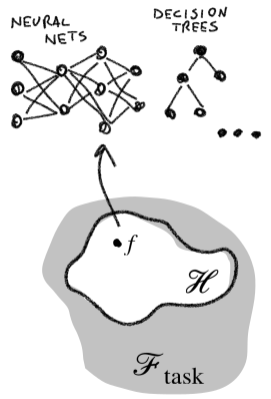
\includegraphics[width=3cm, height=4.5cm]{img/hyp_space.png}
\end{minipage}
	
	
\bigskip

In order to learn a function \(f \in \mathcal{F}_{task}\) we have to minimize a (generalization) error function \(E(f;P_{data})\). The error function determines how well a solution \(f \in \mathcal{F}_{task} \) fits some given data. It guides the selection of the best solution in \(\mathcal{F}_{task}\)

\bigskip

The ideal target function is given by \(f^\star \in \underset{f \in \mathcal{F}_{task}}{\arg\min} \quad E(f; P_{data})\). Too large search space and we need a feasible way of implementation. So, we need to restrict the search space (hypothesis space).
\bigskip


We need to restrict the focus on finding functions that can be implemented and evaluated in a tractable way. We define a model hypothesis space \(\mathcal{H} \subset \mathcal{F}_{task}\) and seek a solution within that space.

The feasible target function is given by \(f^{\star}_{\mathcal{H}} \in \underset{f \in \mathcal{H}}{\arg\min} \quad E(f; P_{data})\). This feasible target function is still problematic, because we cannot be computed exactly as \(P_{data}\) is unknown.

\bigskip

	
Wee need to work on a training set \(\mathcal{D}_n = \{z_1, ..., z_n\}\) where \(z_i = (x_i, y_i) \in \mathcal{X} \times \mathcal{Y}\) and \((x_i, y_i)\) are the input and the output \emph{z}, sampled from \(P_{data}\).

The actual target function in given by \(f^{\star}_{\mathcal{H}}(\mathcal{D}_n) \in \underset{f \in \mathcal{H}}{\arg\min} \quad E(f; D_n)\), where \(E(f; D_n)\) is the training error. It is no longer minimization of the generalization error, but now it is minimization of the training error.


\subsection*{Error function}

Typically, the generalization and training error functions can be written in terms of a pointwise loss \(\mathcal{l}(f;z)\) measuring the error incurred by \emph{f} on the training example \emph{z}

\(E(f; P_{data}) = \mathbb{E}_{z\sim P_{data}} [l(f;z)] \qquad\longrightarrow\) generalization error


\(E(f; D_n) = \dfrac{1}{n} \sum l(f; z_i) \qquad \longrightarrow\) training error

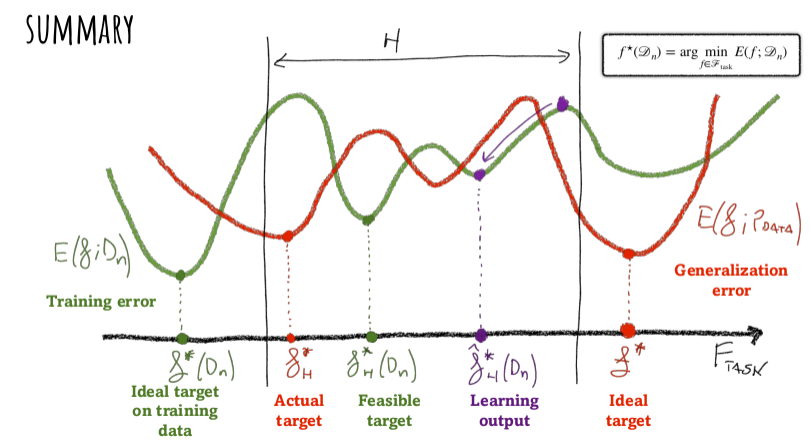
\includegraphics[width=15cm, height=8cm]{img/summary2.png}



\subsection*{Errors}
\textbf{Underfitting. } We have a large error on the training set. The ideal target is far away from the learning output.

\textbf{Overfitting.} There is a small training error, but a very high generalization error. The model fits the data too well and cannot be generalized on other data sets

The \textbf{estimation error} is an error induced by learning on a data sample, while an \textbf{approximation error} is an error induced by the hypothesis space \(\mathcal{H}\). An \textbf{irreducible error} is an error due to inherent variability in the data


In order to improve generalization we can avoid to attain the minimum on training error, reduce the model capacity (e.g. not having polynomial with very high degree, then possibility of overfitting decreases); change the objective function and appending to the error with a regularization term. 

We can inject noise in the learning model and/or stop the learning algorithm before convergence (early stopping).

Also, we can increase the amount of data adding more training samples and/or augmenting the training set with transformations; combine predictions from multiple, de-correlated models and then ensemble the solution (e.g. apply one model to a subset of training data and another model to the (other) subset of data and then merge their predictions)

\subsection*{Regularization}

\begin{minipage}{0.35\linewidth}
Regularization is the modification of the training error function by appending a term \(\Omega(f)\) that typically penalizes complex solutions
\end{minipage}
\hfil
\begin{minipage}{0.55\linewidth}
	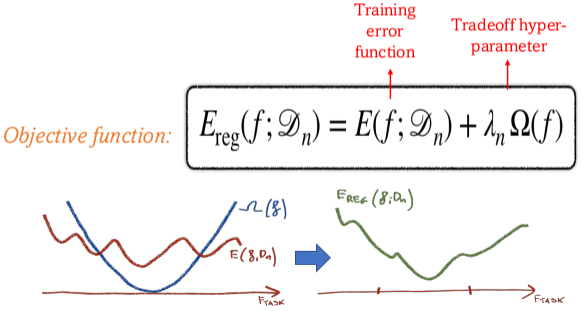
\includegraphics[width=8cm, height=4cm]{img/regularization.png}
\end{minipage}

\bigskip

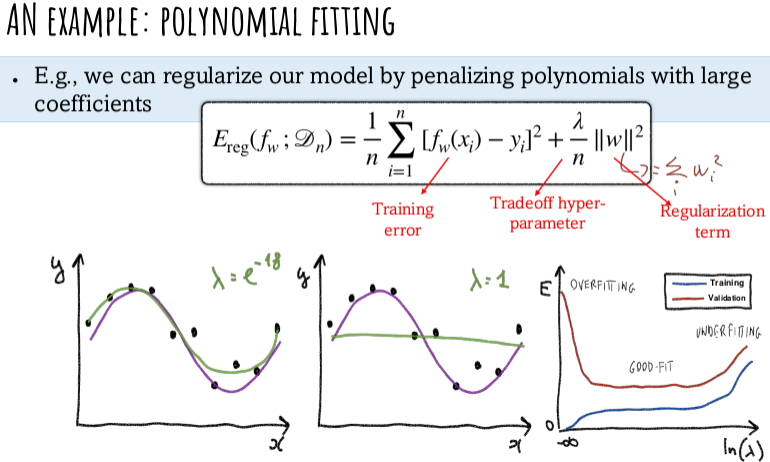
\includegraphics[width=12cm, height=6cm]{img/pol_fitting.png}


\newpage


\section*{7th March}

Features are how our algorithms "view" the data. They are the questions we can ask about the samples. Features are in general represented with (fixed size) vectors.
Given the samples, we map them with the features.


We can turn categorical features into numerical values. Samples are points in an \emph{n}-dimensional space, where \emph{n} is the number of features.

For example, we can plot apples and bananas with \emph{A} and \emph{B} considering as \emph{x} and \emph{y} values, weight and color respectively.

\bigskip


\subsection*{Classification algorithm}

\begin{minipage}{0.5\linewidth}
To classify a sample \emph{d}, we can label it with the label of the closest sample in the training set

To classify a sample \emph{d}, we can find \emph{k} nearest neighbors, and choose \emph{d}'s label as the label which is the majority label within the \emph{k} nearest neighbors.

In order to compute the nearest, we can use distance functions: Euclidean distance, Mahalanobis distance.
\end{minipage}
\hfill
\begin{minipage}{0.45\linewidth}
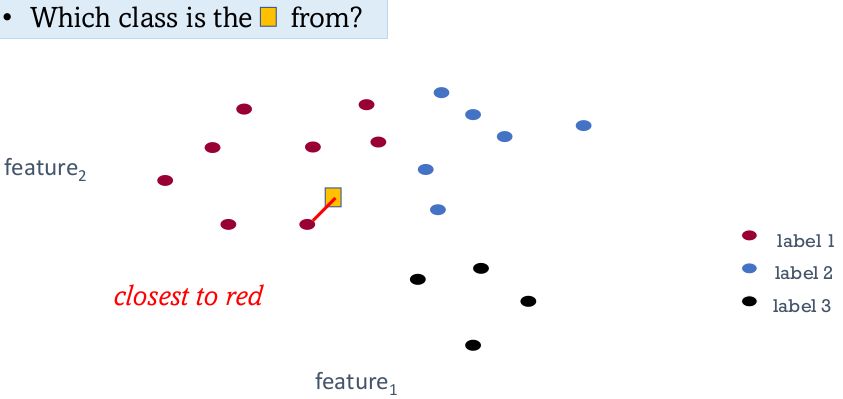
\includegraphics[width=8cm, height=4.5cm]{img/classification.png}
\end{minipage}


\subsubsection*{Euclidean distance}
Given two samples, \emph{p} and \emph{q}, in \emph{n}-dimensional feature space, we have that the distance is
\[d(p, q) = \sqrt{\sum (q_i - p_i)^2}\]

where \(p_i\) and \(q_i\) are the features. What we do is compare each (same) feature of the two samples.


\subsubsection*{Mahalanobis distance}
Centroid is the mean position of all the data points in all directions. For example, given \emph{X} and \emph{Y}, we have that \(centroid=(\overline{X}, \overline{Y})\).

The Mahalanobis distance is a distance measure between a point and a distribution. It takes into account the correlation between variables.



Covariance matrix is computed based on the green data points (similar to how we computed the centroid). Then, calculate the inverse of the covariance matrix.

\[MD = \sqrt{(\overrightarrow{x} - \overrightarrow{\mu})^TS^{-1} (\overrightarrow{x} - \overrightarrow{\mu})}  = \sqrt{\left(\begin{array}{c}
		x - \overline{x}\\
		y - \overline{y}
		\end{array}\right)^T S^{-1} \left(\begin{array}{c}
		x - \overline{x}\\
		y - \overline{y}
		\end{array}\right) }\]

where \emph{x} is the data coordinate, $\mu$ is the centroid, and \emph{S} is the covariance matrix.


\bigskip\bigskip


\begin{minipage}{0.65\linewidth}
\textbf{Decision boundaries} are places in the feature space where the classification of a point/sample changes. The k-nearest neighbor dives locally defined decision boundaries between classes
\end{minipage}
\hfill
\begin{minipage}{0.3\linewidth}
	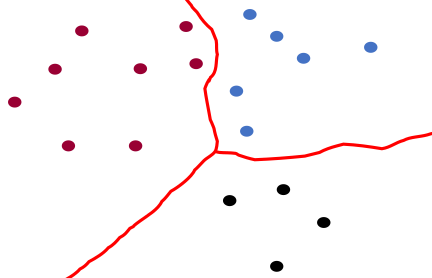
\includegraphics[width=3cm, height=2cm]{img/decision_boundary.png}
\end{minipage}



\bigskip\bigskip

The factors determining how well a machine learning algorithm will perform are its ability to: make the training error small; make the gap between training and test error small.
These two factors correspond to the cases of underfitting and overfitting.
Underfitting occurs when the model is not able to obtain a sufficiently low error value on the training set. Overfitting occurs when the gap between the training error and test
error is too large.


\bigskip


\textbf{How to decide k of k-NN?} We can use common heuristic: often we choose 3, 5 or 7, or we can choose in general an odd number to avoid ties.

Otherwise, we can use the training and validation data (that never overlap) to decide \emph{k}. We change \emph{k} from \(k=1\) until the validation performance decreases. We have to pay attention to not underfit or overfit the data. Then we have to finalize the decision of \emph{k} and use the same \emph{k} to classify the test data.

\bigskip

A variation of k-NN is the weighted k-NN, in which we assign a weight (or vote) to the samples so that closer samples have more weight. When distance increases, the weight decreases. If a point is far from \emph{k} points, then the weight will be lower, and the point is likely to be not in the same group with the other points. 

One possible weight function could be \(weight = F(distance) = \dfrac{1}{distance}\). \\

The class of the test data is predicted based on the weighted sum, not on majority vote as in k-NN


\subsubsection*{K-NN, pros and cons}
The main advantage of using k-NN is that we do not need almost no assumptions about the data. Smoothness: nearby regions of space are from the same class. And the assumptions implied by distance function (only locally!). It is a non-parametric approach, and the only thing we have to infer from the data is \emph{k}. Also, it is easy to update in online setting: just add new item to training set.

There are some disadvantages: we need to handle missing data; it is sensitive to class-outliers and to lots of irrelevant attributes (affect the distance); it is computationally expensive in terms of space (need to store all the training samples) and time (need to compute distance to all samples - O(nd)).




\subsection*{Decision Trees}

A decision tree is a tree-structured, prediction model. It is composed of terminal (or leaf)  nodes and non-terminal nodes. Non-terminal nodes have 2 or more children and implement a routing function. Leaf nodes have no children and implement a prediction function. There are no cycles, all nodes have at most 1 parent excepting root node.

A decision tree takes an input \(x \in \mathcal{X}\) and routes (traverse) it through its nodes until it reaches a leaf node. In the leaf a prediction takes place.

Each non-terminal node \(Node(\phi, t_L, t_R)\) holds a routing function \(\phi \in \{L, R\}^{\mathcal{X}}\) such that there exist a left child \(t_L\) and right child \(t_R\).

When \emph{X} reaches the node it will go to the left child or the right child depending on the value of \(\phi(x) \in \{L, R\}\).


Each leaf node holds a prediction function \(h \in \mathcal{F}_{task}\) (typically a constant). Depending on the task we want to solve it can be \(h \in \mathcal{Y}^\mathcal{X}\), e.g. classification or regression or density estimation. Once \emph{X} reaches the leaf the final prediction is given by \(h(x)\).



The decision tree function is given by
\[f_t(x) = \left\{ \begin{array}{ll}
h(x) & \text{ if } t = Leaf(h)\\
f_{t_{\phi(x)}}(x) & \text{ if } t = Node(\phi, t_L, t_R)
\end{array}\right.\]

If we are in a leaf, we make a prediction. Otherwise we have to decide with \(f_{t_{\phi(x)}}(x)\) where to go, left or right.

\centering
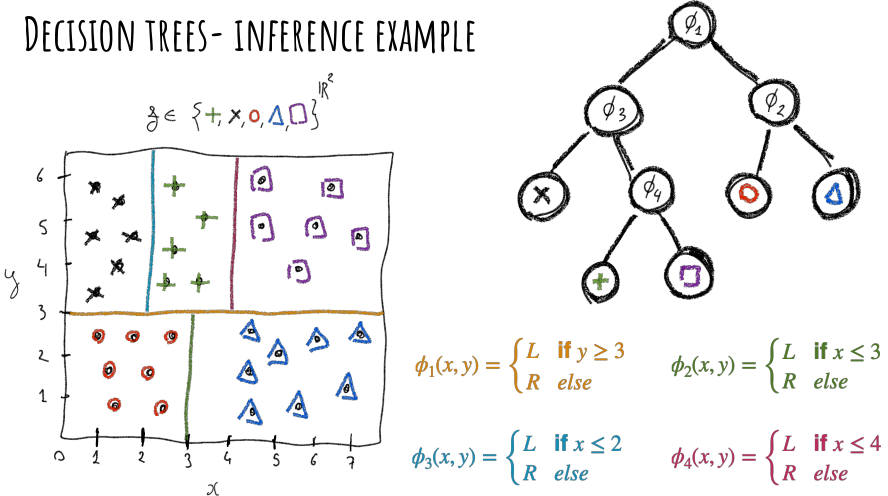
\includegraphics[width=13cm, height=7cm]{img/decision_tree.png}


\bigskip

\raggedright Given a training set \(\mathcal{D}_n = \{z_1, ..., z_n\}\) we want to find a tree \(t^{\star}\)

\[t^\star \in  \underset{f \in \mathcal{T}}{\arg\min}E(f_t; \mathcal{D}_n)\]

This optimization problem has many solutions. Thus we need to impose constraints, e.g. most compact tree, otherwise it could be NP-hard

We need to fix a set of leaf predictions \(\mathcal{H}_{leaf} \subset \mathcal{F}_{task}\) (e.g.
constant functions). Fix a set of possible splitting functions \(\Phi \subset\{L, R\}^\mathcal{X}\). Tree-growing strategy recursively partition the training set and decides whether to grow the leaves or non-terminal nodes: ID3 algorithm by Ross Quilan, CaRT by Breiman et al.




\subsubsection*{ID3 algorithm}

Split(node, \{examples\}): \(\qquad\longrightarrow\) Operates on each node in the tree. For each node you get a subset training examples that falls into that node
\begin{enumerate}
	\item A $\leftarrow$ the best attribute/feature for splitting the \{examples\}
	\item Decision attribute for this node  $\leftarrow$ A
	\item For each value of A, create new child node \(\qquad \longrightarrow\) if A has 3 possible values, then there are 3 children
	\item Split training \{examples\} to child nodes
	\item For each child node/subset: if subset is not pure, then split(child\_node, \{subset\})
\end{enumerate}


\textbf{How to pick the best feature?} We want to measure the purity of the split. A pure set is a set where we are 100\% sure to have a certain value, impure otherwise. There are different ways to measure the purity (e.g. entropy)

Assume that we have binary classes (positives and negatives), where p(+) is the proportion of positives in a subset, and p(-) is the proportion of negatives in a subset. The entropy of a subset is given by \(H(s) = - p_{(+)}log_2p_{(+)} - p_{(-)}log_2p_{(-)}\). The subset with bigger entropy is less pure.

\bigskip

\textbf{Information gain. } We want to have many items in the pure sets. We calculate the expected drop in entropy after each split.
\[Gain(S, A) = H(S) - \sum \dfrac{|S_v|}{|S|}H(S_v)\]

where \emph{v} is the possible values of A, \emph{S} is the set of samples \(\{X\}\), and \(S_v\) is the subset where \(X_A = V\). There is mutual information between A and class labels of S. 
We use information gain to decide which attribute to pick, we want to maximize the "information gain"
\bigskip

\textbf{Information gain.  }We use information gain to decide which attribute to pick. First, we take every attribute in the data, compute gain for that attribute and select the attribute that has the highest information gain (that's the attribute which reduce the uncertainty the most, aka lead the purest possible split out of all attributes). 
We consider one level split at a time, but remember that the procedure is recursive.
\bigskip



Decision trees are non-parametric models with a structure that is determined by the data. As a result, they are flexible and can easily fit the training set, with high risk of overfitting. Standard techniques to improve generalization apply also to decision trees (early stopping, regularization, data augmentation, complexity reduction, ensembling). A technique to reduce complexity a posteriori is called pruning.

\[Gain\quad Ration (S,A) = \dfrac{Gain(S,A)}{SplitEntropy(S, A)}\]

\[SplitEntropy(S,A) = - \sum \dfrac{|S_v|}{|S|} log \dfrac{|S_v|}{|S|}\]

\bigskip

We can use decision trees also to investigate continuous attributes. We pick a threshold to create a split (e.g. \(temperature > 77.8 = TRUE\))

\bigskip


\textbf{Multi-class classification.} In multi-class classification we have k different classes. The decision tree predict the most frequent class in the subset. The entropy is given by \(H(s) = - \sum_cp_clog_2p_c\), where \(p_c\) is the proportion of the examples of class c in subset S
\bigskip

\textbf{Decision tree - pros and cons. } Pros: interpretable (humans can understand the reason of decision); easily handles irrelevant data (Gain=0); can handle missing data; very compact; very fast at testing time (O(depth)). 

Cons: greedy (may not find best tree) - not globally optimal; exponentially many possible trees; only axis-aligned splits of data (especially in continuous data)


\subsubsection*{Random forest}
Random forests are ensembles of decision trees. Each tree is typically trained on a bootstrapped version of the training set (sampled with replacement).

\centering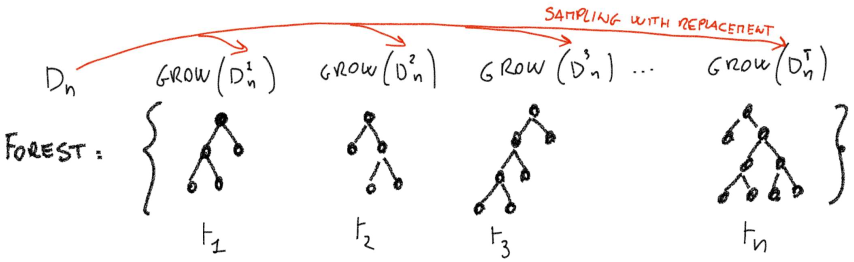
\includegraphics[width=10cm, height=3.5cm]{img/rnd_forest.png}	

\raggedright Split functions are optimized on randomly sampled features or are sampled completely at random (extremely randomized trees). This helps obtaining decorrelated decision trees. The final prediction of the forest is obtained by averaging the prediction of each tree in the ensemble \(\mathcal{Q} = \{t_1, ..., t_T\}\)
\[f_\mathcal{Q}(x) = \dfrac{1}{T} \sum f_t(x)\]


\subsubsection*{Decision tree-summary}
ID3: grows decision tree from the root to down; greedily selects next best attribute using GAIN; entropy is how uncertain we are of Yes/No in a set; information Gain is the reduction in uncertainty following a split. 

Searches a complete hypothesis space; prefers smaller trees, high gain at the root; overfitting addressed by post-pruning; prune nodes, while accuracy increases on validation set; fast, compact, interpretable




\subsection*{The importance of validation set}

The validation set is separate from the training set. It s used to pick algorithm and to decide the parameters of the algorithm. The best performing algorithm with knob settings; fine-tuning knobs (e.g., the depth of the trees, k of k-NN….)


ATTENTION: splitting the datasets into training, validation and testing can be done randomly to avoid BIAS. There can be some specific rules to apply.

\subsection*{Cross validation}

When you split the dataset: training, validation, testing, you can have conflicting priorities.
\begin{itemize}
	\item Estimate future error (i.e., testing error) as accurately as possible by making the test set as big as possible. (High confidence interval)
	\item Learn classifier as accurately as possible by making the training set as big as possible. (Better estimates, maybe better generalization)
	\item Training and testing instance CANNOT OVERLAP
\end{itemize}

Training and testing cannot overlap, but \(n_{train} + n_{test} = constant\)

The cross validation idea is: Train $\rightarrow$ Test, then swap the data, hence we train the test data and test on the train data (Test $\rightarrow$ Train, and average results).

At each fold (step) you use each instance only in one set, so no overlapping. If there are two folds, you have two models trained. Every sample is in both training and testing but not at the same time. It reduces the chances of getting an biased training set

\subsubsection*{Fold cross validation}
We randomly split the data into 5 folds, then test on each fold while training on 4 other folds (80\% train, 20\% test). Then average the result over 5 folds.


\centering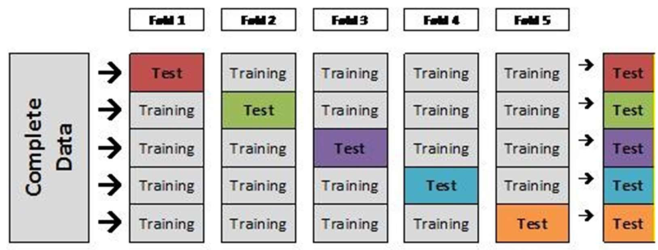
\includegraphics[width=10cm, height=4.5cm]{img/cross_validation.png}	

\raggedright	
\subsubsection*{Leave-one-out cross validation}

We have n-fold cross validation. We train on all (n-1) samples, while test on 1 instance. It is the best possible classifier since it learned from n-1 training samples. On the other hand, it has hogh computational cost (re-learn everything for \emph{n }times), and the classes are not balanced in training/testing set, but we have a solution: \textbf{stratification}.
\bigskip

\textbf{Stratification.} Keep class labels balanced across training and testing sets. Instead of taking the dataset and dividing it randomly into \emph{K} parts, we take the dataset, divide it into individual classes. Then for each class, divide the instances in \emph{K} and assemble ith part from all classes to make the ith fold (attention! It is still random).

\subsection*{Evaluation measures}
	
We use evaluation measures to decide if our model is performing well. To decide out of many models, which performs better than the other, we can use accuracy, training error, ...

In classification tasks we consider how often we classify something right/wrong. In regression how close are we to what we are trying to predict. In clustering how well do we describe our data (in general, very hard)
	

\centering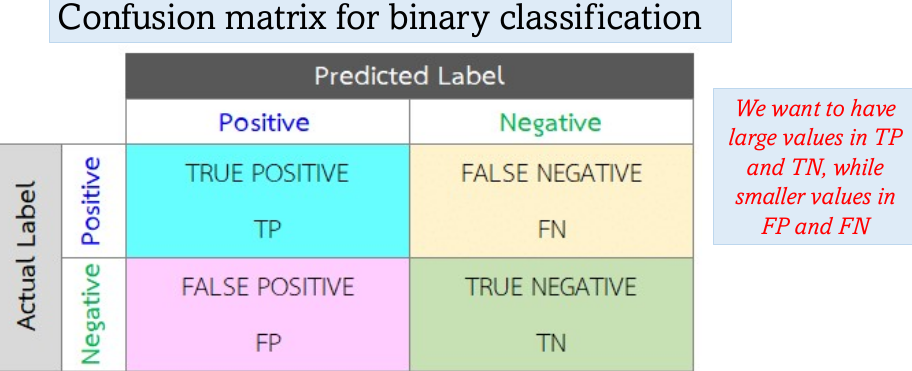
\includegraphics[width=10cm, height=4.5cm]{img/confusion_matrix.png}	

\raggedright Classification error \( = (fp + fn) / (tp + tn + fp + fn)\)

Accuracy \(= (1 - error) = (tp + tn) / (tp + tn + fp + fn)\)

These are basic measures of goodness of a classifier. But we have to pay attention, since it is very misleading if we have imbalanced classes.



\centering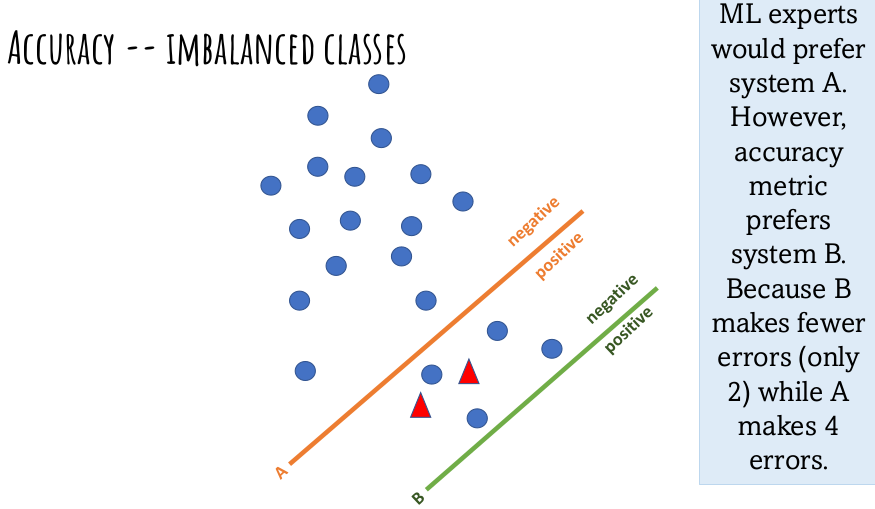
\includegraphics[width=13cm, height=7cm]{img/accuracy.png}	


\bigskip
\raggedright False Alarm Rate = False Positive Rate = \(FP / (FP+TN)\). It is \% of negative we misclassified as positive

Miss rate = False Negative Rate = \(FN / (TP+FN)\). It is \% of positives we misclassified as negative

Recall = True Positive Rate = \(TP / (TP+FN)\). \% of positives we classified correctly (1-miss rate)

Precision = \(TP / (TP+FP)\). \% positive out of what we predicted was positive



\subsubsection*{Cost of the task}

We typically do not use the evaluation metrics: accuracy, recall, precision etc. alone but instead declare a couple of them together. However, especially in order to optimize a learner automatically (i.e., training), we need a single evaluation measure. The single metric domain specific, so it depends on the task. Depending on the cost of the task we can decide whether we take care more on having less false positives or less false negatives through weighting them.

\[Cost = C_{FP} * FP + C_{FN} * FN\]


\textbf{F-measure}
\[F_1 = 2 * \dfrac{precision * recall}{precision + recall}\]

which is the harmonic mean of precision and recall. The \(F_1\) measure is a sort of accuracy without the true negative. It is used frequently in information retrieval systems




\bigskip
\subsection*{Regression evaluation methods}

In classification we can count of often we are correct or wrong in our predictions. In regression we cannot count, predicting \(y_i\) (continue value) from inputs \(x_i\). Here the question is not \emph{how many times the method is wrong} but \emph{how much the method is wrong wrt. to the truth-labels}

\textbf{Root MSE. } It is a popular and nicely differentiable, but it is sensitive to single large errors (outliers), and very sensitive to single large deviations in the prediction. It is given by
\[\sqrt{\dfrac{1}{n} \sum (f(x_i) - y_i)^2}\] 

where \(\frac{1}{n} \sum \) is the testing set, \(f(x_i)\) is the predicted, and \(y_i\) is the true.

MSE It is very sensitive to the mean and scale of the prediction. Having the right mean matters.


\centering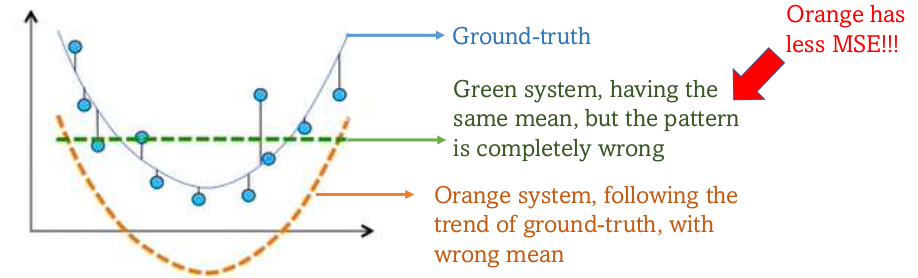
\includegraphics[width=12cm, height=4cm]{img/mse.png}	


\raggedright \# Orange has HIGHER MSE than green.

In order to handle this we can use te relative squared error. MSE is divided by what would happen if you used just the mean as prediction

\[\sqrt{\dfrac{\sum (f(x_i) - y_i)^2}{\sum (\mu_i - y_i)^2}}\]

where \(\sum (f(x_i) - y_i)^2\) is the MSE of predictor, and \(\sum (\mu_i - y_i)^2\) is the MSE when using the mean as a predictor. 


\bigskip

\textbf{Mean absolute error. } It is less sensitive to outliers (a single large deviation will not overpower many small deviations). We take the absolute value since some differences are positive and others are negative, and we do not want them to cancel each other. It is given by
\[\dfrac{1}{n} \sum |f(x_i) - y_i|\]

But, it is not differentiable (you cannot take the derivative of it and taking derivative is important if you want to build an algorithm that minimizes the function.)

\bigskip

\section*{22nd march}

\subsection*{Multiclass classification - evaluation}
Confusion matrix is a generalized version of the binary one. nij is the number of examples with actual
label \(y_i\) and predicted as \(y_j\). The main diagonal contains true positives for each class. The sum of off-diagonal elements along a column is the number of false positives for the column label. The sum of off-diagonal elements along a row is the number of false negatives for the row label.

\[FP_i - \sum\limits_{j \neq i} n_{ji}\qquad \qquad FN_i - \sum\limits_{j \neq i} n_{ij}\]

Accuracy, precision, recall and F1-measure carry over to a per-class measure considering as negative examples from other classes.

\[Pre_i = \dfrac{n_{ij}}{n_{ij} + FP_i} \qquad Rec_i = \dfrac{n_{ij}}{n_{ij} + FN_i}\]


Multiclass accuracy is the overall fraction of correctly classified. examples:

\[MAcc = \dfrac{\sum n_{ij}}{\sum \sum n_{ij}}\]


\subsection*{Feature selection}


\begin{minipage}{0.45\linewidth}
The process of selecting the input variable to your model by using only relevant data and getting rid of "noise" in data. Because, the noisy (irrelevant) attributes can mislead your model, thus decrease its performance.

\end{minipage}
\hfill
\begin{minipage}{0.45\linewidth}
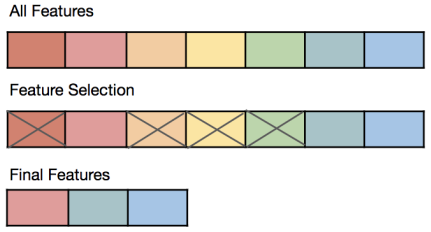
\includegraphics[width=6cm, height=3cm]{img/task_selct.png}	
\end{minipage}


High dimensional data suffers from \emph{Curse of Dimensionality}: observations in a high-dimensional space are more sparse and less representative than those in a low-dimensional space. Using feature selection, we can optimize our model in several ways: prevent learning from noise (overfitting); improved performance, e.g., accuracy, precision, etc.; reduce training time (more features, typically means more training time).

\bigskip

\begin{minipage}{0.45\linewidth}
	\centering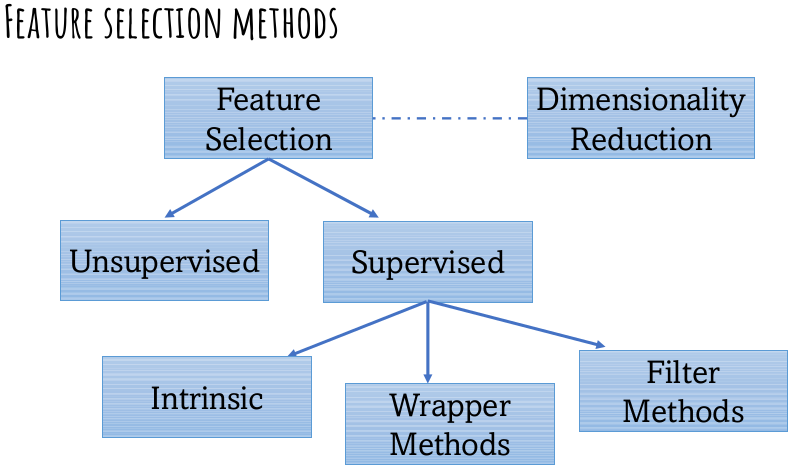
\includegraphics[width=8cm, height=5cm]{img/feat_selection.png}	
\end{minipage}
\hfill
\begin{minipage}{0.45\linewidth}
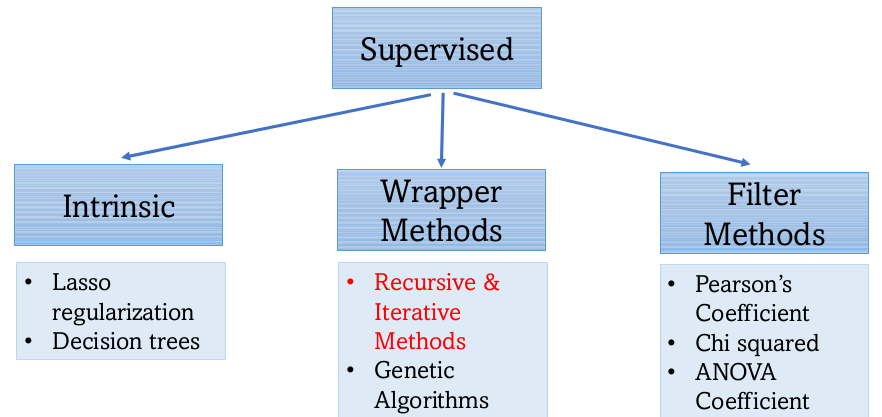
\includegraphics[width=8cm, height=4cm]{img/feat_selection2.png}	
\end{minipage}


\bigskip
\raggedright \emph{Forward feature selection} is an iterative method in which we start with having a single feature in the model. In each iteration, we keep adding the feature which improves our model the most, till an addition of a new variable does not improve the performance of the model.
\bigskip

\begin{minipage}{0.45\linewidth}
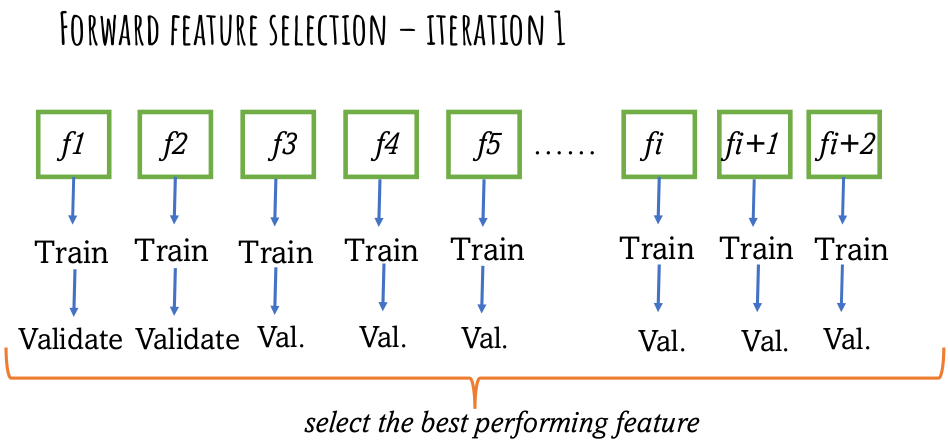
\includegraphics[width=8cm, height=4cm]{img/feat_selection3.png}
\end{minipage}
\hfill
\begin{minipage}{0.45\linewidth}
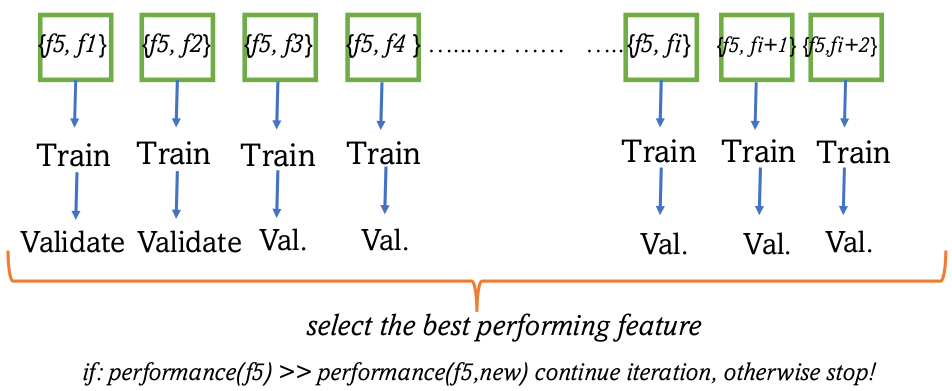
\includegraphics[width=9cm, height=4cm]{img/feat_selection4.png}	
\end{minipage}

In the second iteration keep the selected feature constant, and check if any of the other features is better the chosen one. If there is one, start again, otherwise continue the iteration.

\bigskip\bigskip

\centering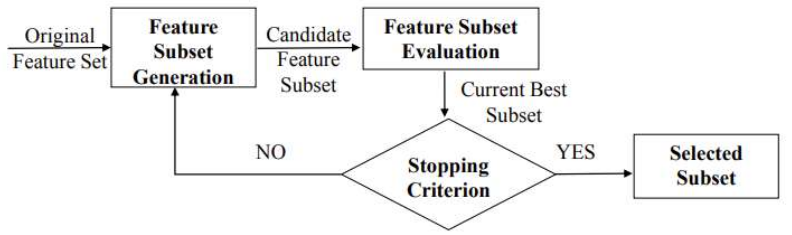
\includegraphics[width=10cm, height=3.5cm]{img/feat_selection5.png}	

	
\raggedright \emph{Backward feature selection} is an iterative method in which we start with all features, and we remove the least significant feature at each iteration such that removing it increases (rarely not changes) the performance of the model. We repeat this until no improvement is observed on removal of features.

\bigskip\bigskip


\subsection*{Support vector machines}

\textbf{Binary classification recap. }Given a training data \((x_i, y_i)\) for \(i=1, ..., n\) with \(x_i \in \mathbb{R}^d\), and \(y_i \in \{-1, 1\}\) learn a classifier \(f(x)\) such that
\[f(x_i) \left\{\begin{array}{ll}
\geq 0 & y_i = 1\\
< 0 & y_i = -1
\end{array}\right.\]

\bigskip

\textbf{Linear separability}

\centering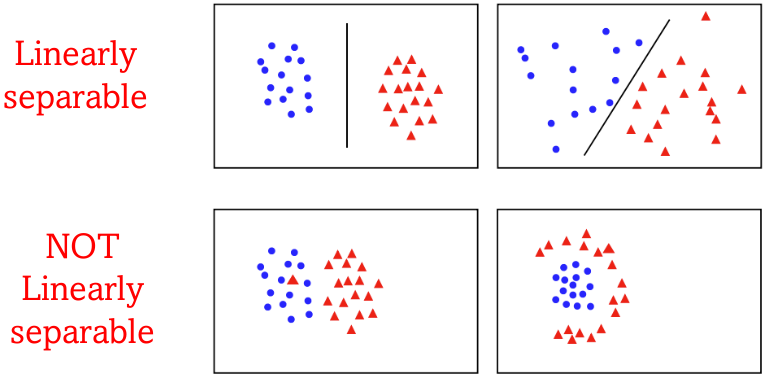
\includegraphics[width=9cm, height=3.5cm]{img/lin_class.png}	


\raggedright A \emph{linear classifier} has the form \(f(x) = w^Tx+b\). In the 2-dimension, the discriminant is a line, in the 3-dimension is a plane, and in n-dimension is an hyperplane. \emph{W} is the normal to the line, and it is called \emph{weight vector}, while \emph{b} is the bias.

In linear classifier, the training data is used to learn \emph{W} (we ignore the training data after learning \emph{W}) Only \emph{W} is needed to classify the validation/test data. 




The margin of a classifier is the distance to the closest points of either class. Large margins classifiers attempt to maximize this. What we want to do is to maximize the margin.

For any separating hyperplane, there exist some set of "closest points", the \emph{support vectors} (representative of the data). For \emph{n} dimensions, there will be at least \(n+1\) support vectors.

Maximizing the margin is good since it implies that only support vectors matter, other training examples are ignorable.

\bigskip
\begin{minipage}{0.45\linewidth}
The margin is the distance to the support vector. That is, the distance between the representative points, on either side of the hyperplane.
\end{minipage}
\hfill
\begin{minipage}{0.45\linewidth}
	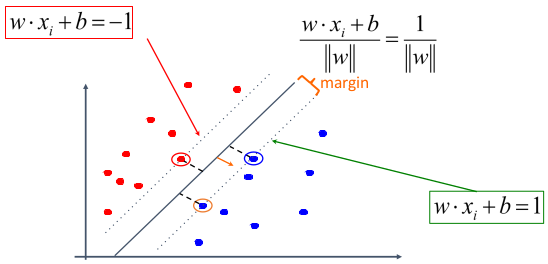
\includegraphics[width=7cm, height=4cm]{img/margins.png}	
\end{minipage}

In order to maximize the margin, we select the hyperplane with the largest margin where the points are classified correctly and outside the margin.This is setting up as a \emph{constrained optimization problem}. Maximizing the margin is equivalent to minimize the norm of the weights, subject to separating constraints.

\[max_{w, b} margin(w, b) \longrightarrow max_{w, b} \dfrac{1}{||w||} \longrightarrow min_{w, b} ||w||\]

that are subject to \(y_i(w\cdot x_i+b)\geq 1 \forall i\). The minimization criterion wants \emph{w} to be as small as possible. The constraint make sure that the data is separable. 
\bigskip
	
\subsubsection*{Support vector machine (SVM)}

Support vector machine problem is a version of a quadratic optimization problem. Maximizing or minimizing a quadratic function subject to a set of linear constraints.

How SVM really works: find a boundary vector \emph{w} for a data \(d_{i, j}\) (=\emph{x}) that satisfies condition:


\begin{minipage}{0.45\linewidth}
\begin{itemize}	
	\item \(\sum w_i d_{i, j} \geq 1 \longrightarrow\) all positive get scores \(\geq 1\) 
	\item \(\sum w_i d_{i, j} \leq -1 \longrightarrow\) all negative get scores \(\leq -1\) 
	\item \(min||w|| \longrightarrow\) maximum margin around \emph{w}
\end{itemize}
\end{minipage}
\hfill
\begin{minipage}{0.45\linewidth}
	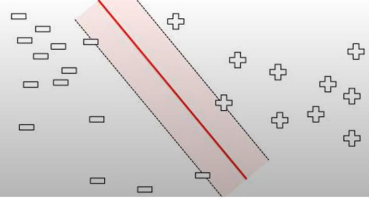
\includegraphics[width=6cm, height=3cm]{img/svm.png}	
\end{minipage}



where \(\vec{w} = \sum \alpha_j, \vec{d}_j - \sum \alpha_j\vec{d}_j\).

\bigskip

There is an analogy with centroids: if \(\alpha_j = 1/\)n of the positive and negative, respectively, then \( \sum \alpha_j, \vec{d}_j\) is the centroid of positives, while \(- \sum \alpha_j, \vec{d}_j\) is the centroid of negatives.

However, instead we have some weights \(\alpha_j\), meaning that we give more weights to some data points, and less weights to some others. Importantly, most of the $\alpha_j$ is zero, but the only one that matters are the ones on the boundary.

\bigskip

\textbf{Convex Hull}: draw polytope (area) around all positives/negatives. Any point \emph{h} in the polytope is a linear combination of corner data points: \(\vec{h} = \sum \alpha{hd} \vec{d}\). Any point in the polytope can be obtained from the corner points. What we have to find are the two nearest points \emph{h+} and \emph{h-}. 

The margin must be \(||h+ - h-||\), the distance between \emph{h+} and \emph{h-}. The margin cannot be bigger o smaller that the difference between the positives and the negatives. The boundary must be half-way along \(h+ \text{ and } h-\), and it must be perpendicular to this distance-line to be able to maintain the margins. Hence, \(\vec{w} = \sum \alpha_j, \vec{d}_j - \sum \alpha_j\vec{d}_j\)
	
\bigskip 

Sometimes happens that we have a problem in which the constraints do not allow to solve it, maybe since we have some data point in the wrong side. For this reason we define a \emph{slack variable}, \(min_{w, b} ||w||^2 + c\sum_i \sigma_i\), with $\sigma_i \geq 0$ for each sample. This variable allows us to make mistakes.


Every constraint can be satisfied if the slack variable is sufficiently large. \emph{C} is a regularization parameter: if it is small (large margin) the constraints can be ignored; if it is large (narrow margin) the constraints are hard to ignore. If \emph{C} goes to $\infty$, it enforces all constraints and we have hard margins.

The slack variable changes between data points. The slack values for points outside (or on) the margin and correctly classified is zero. The slack variable have to be greater than or equal to zero and if they are on or beyond the margin, then \(y_i(wx_i + b) \geq 1\) is already satisfied. 

The slack value for points inside the margin and classified correctly is the difference from the point to the margin: \(\delta_i = 1 - y_i (w \cdot x_i + b)\). The slack values for points that are incorrectly classified is the distance to the hyperplane plus the distance to the margin. \emph{Distance} is the unnormalized projection \( - y_i(w \cdot x_i+b)\), not to be confused with the true distance, which would be with respect to \(w/||w||\)

\[\delta_i = \left\{\begin{array}{ll}
0 & if \quad y_i(w \cdot x_i + b) \geq 1\\
1 -  - y_i(w \cdot x_i+b) & otherwise
\end{array}\right.\]

\textbf{Losses }
\begin{itemize}
	\item Hinge: \(l(y, y') = max(0, 1 - yy')\)
	\item Squared loss: \(l(y, y') = (y-y')^2\)
	\item 0-1 loss: \(l(y, y') = 1[yy\ \leq 0]\)
\end{itemize}


\textbf{Soft margin. } \(min_{w, b} ||w||^2 + X \sum loss_{hinge}(y_i, y_i')\)



\bigskip

\subsubsection*{Summary}

The classifier is a separating hyperplane. The most important training points are support vectors; they define the
hyperplane. A quadratic optimization problem, also referred as primal problem. One possible way to solve quadratic optimization problems involves constructing a dual problem where a Lagrange multiplier $\alpha_i0$ is associated with every inequality constraint in the primal (original) problem. Quadratic optimization algorithms can identify which training points are support vectors with non-zero Lagrangian multipliers $\alpha_i$.

\bigskip 

Dual problem: find \(\alpha_1, ..., \alpha_n\) such that \(Q(\alpha) = \sum_{\alpha_i} - 1/2 \sum_{alpha_i, y_i} \sum_{alpha_j, y_j} x_i^Tx_j\) is maximized, and \(\sum_{\alpha_i, y_i} = 0\) and \(\alpha_i \geq 0 \forall \alpha_i\). 

Given a solution \(\alpha_1, ..., \alpha_n\) to the dual problem, the solution to the primal is: \[w = \sum \alpha_i y_i x_i \qquad b = y_k - \sum \alpha_i y_i x_i^Tx_k \text{ for any } \alpha_k > 0\]

Each non-zero $\alpha_i$ indicates that the corresponding \(x_i\) is a support vector.

Then the classifying function is \[f(x) = \sum \alpha_i y_i x_i^Tx+b\]

The solution relies on an inner product between the test point \emph{x} and the support vector \(x_i\). Also solving the optimization problem involved computing the inner products between all training points.


If we have not separable case Dual problem: find \(\alpha_1, ..., \alpha_n\) such that \(Q(\alpha) = \sum_{\alpha_i} - 1/2 \sum_{\alpha_i, y_i} \sum_{\alpha_j, y_j} x_i^Tx_j\) is maximized, and \(\sum_{\alpha_i, y_i} = 0\) and \(0 \geq \alpha_i \geq C \forall \alpha_i\). Also here, \(x_i\) with non-zero $\alpha_i$ will be support vectors


\bigskip



\subsection*{Non-linear SVM}
Datasets that are linearly separable with some noise work out great. However, what we can do if the dataset is too hard? Instead of relying on a 2-dimensional spoace, we map data to a higher-dimensional space.

The general idea is: the original feature space can always be mapped to some higher-dimensional feature space where the training set is separable. Hence, what we have to do is find a function \(\Phi: x \rightarrow \phi(x)\)

\subsubsection*{Kernel Trick}
The linear classifier relies on inner product between vectors: \(K(x_i, x_j) = x_i^Tx_j\). If every data point is mapped into high dimensional space via some transformation $\Phi$: \(x \rightarrow \phi(x)\), the inner product becomes:  \(K(x_i, x_j) = \phi(x_i)^T\phi(x_j)\). A kernel function is a function that is equivalent to an inner product in some feature space.

A kernel function implicitly maps data to a high-dimensional space, without the need to compute each \(\phi(x)\) explicitly.

When you run SVM we have to choose the correct kernels for the type of data:
\begin{itemize}
	\item Linear: \(K(x_i, x_j) = x_i^Tx_j\)
	\item Polynomial of power \emph{p}:  \(K(x_i, x_j) = (1 +x_i^Tx_j)^p\)
	\item Gaussian:  \(K(x_i, x_j) = e^{- \frac{||x_i - x_j||^2}{2 \sigma^2}}\)
		\subitem mapping $\Phi$: \(x \rightarrow \phi(x)\), where $\phi(x)$ is \emph{infinite-dimensional}: every point is mapped to a Gaussian function; combination functions for support vectors is the separator
	\item Higher-dimensional space still has intrinsic dimensionality \emph{d} (the mapping is not onto), but linear separators in it correspond to non-linear separators in the original space.
\end{itemize}


\bigskip

Support vector machines are still among the best performers for several classification tasks ranging from text to genomic data. They can be applied to complex data types beyond features vectors by designing kernel functions for such data. SVM have been extended to several tasks such as regression, PCA, etc.
	










\section*{24th march (?)}

The aim of \emph{dimensionality reduction} is to represent samples with fewer variables while preserving the structure of the data as much as possible. The discriminative is that keep only structure that affects class separability.

\subsection*{Principal component analysis}

The most frequently used method to reduce the dimensionality is the \emph{Principal Component Analysis}. PCA defines a set of principal components: the first follows the direction of the greatest variablity of the data; the second component is perpendicular to the first (gratest variability of what is left); ... and so on until we reach \emph{d} (original dimensionality). The first \emph{m} components become \emph{m} new dimensions.

We change the coordinates of every data point to these dimensions, then apply the machine learning algorithm.

\textbf{When use PCA.} If you want to reduce the number of variables, but aren't able to identify variables to completely remove from consideration; if you want ot ensure that your variables are independent of one another; if you are comfortable making your independent variables less interpretable. 

If you don't agree with the last, then you should not use PCA.


\subsubsection*{PCA algorithm}

\begin{enumerate}
	\item get some data
	\item subtract the mean from each dimension $\rightarrow$ this produce a dataset whose mean is zero
	\item calculate the covariance matrix
		\subitem if the data is 2-dimensional, the covariance matrix will be \(2 \times 2\)
		\subitem for 3-dimensional dataset, you can calculate \(cov(x, y), cov(x, z), cov(y, z)\)
		\subitem for n-dimensional dataset you need to compute \(\frac{n!}{(n-2)!*2}\)
	\item compute the eigenvectors and eigenvalues of the covariance matrix \(\rightarrow Av = \lambda v\), where \emph{A} is the matrix, $\lambda$ is the eigenvalue, and \emph{v} is the eigenvector
	\item choose the components and form the new feature vector
		\subitem the eigenvector with the highest eigenvalue is the principal component of the dataset
		\subitem once eigenvectors are found from the covariance matrix, we order them by eigenvalue, highest to lowest, which gives the components in order of significance.
	\item obtain the new dataset
		\subitem chosen the components, we form a feature vector from them, then take the transpose of the vector and multiply it on the left of the original dataset
		\subitem \(FinlData = RowFeatureVector \times RowDataAdjust\)
			\subsubitem \emph{RowFeatureVector} is the matrix with the eigenvectors in the columns transposed so that the eigenvectors are now in the rows, with the most significant eigenvector at the top
			\subsubitem \emph{RowDataAdjust} is the mean-adjusted data transposed, i.e., the data items are in each column, with each row holding a separate dimension.
\end{enumerate}

\textbf{How many principal components?} It depends on the goal and the application. No means of validating it, unless we use it in the context of a supervised method (e.g., reduce the input dimensionality for a supervised algorithm). Nonetheless we can compute the cumulative proportion of $\lambda$ for the first \emph{k} principal components allowing to estimate the amount of information loss. As a threshold one can use 90\%, 95\%, etc.


\subsubsection*{Reminder: eigenvalues and eigenvectors}
	
Eigenvectors are perpendicular to each other. They provide us with information about the patterns in the data. One of the eigenvectors goes through the middle of the points, like drawing a line of best fit. That eigenvector is showing us how these two attributes are related along that line. The second eigenvector gives us the other, less important, pattern in the  data, that all the points follow the main  line, but are off to the side of the main line by some amount.
	
	
	
\subsection*{Clustering}
	
In the \emph{clustering} setting we have raw data, from which we extract features and then group them into groups, or clusters. There is no supervision, we are only given data and want to find groupings. \emph{Clustering} is the process of grouping a set of samples into cluster of similar samples.

We can have hard and soft clustering. In the first case, the clusters do not overlap and the elements either belong to a cluster or not. In the second case, clusters may overlap, and we need to find the strength of association between the element and the cluster, hence how much does a sample belong to a cluster (e.g. based on probability).

Also, we can have flat ot hierarchical clustering: set of groups versus taxonomy.


\bigskip
\subsubsection*{K-means}
The most well-known and popular clustering algorithm is the \emph{K-mean}. It is fine with numerical attributes, but not with categorical attributes. The algorithm works as follow:

\begin{itemize}
	\item Start with initial cluster centers randomly picked $\rightarrow$ the number of cluster = \emph{k}
	\item Iterate (until no sample changes its cluster) and assign/cluster each sample to the closest center (distance calculation); then recalculate the centers of each cluster as the mean of the samples in a cluster
\end{itemize}


\textbf{Distance measures}:
\begin{itemize}
	\item Euclidean distance \(d(x, y) = \sqrt{\sum (x_i - y_i)^2}\)
	\item Cosine similarity \(sim(x, y) = \frac{x \cdot y}{|x||y|} = \frac{x}{|x|} \cdot \frac{y}{|y|} = \frac{\sum x_i y_i}{\sqrt{\sum x_i^2} \sqrt{\sum y_i^2}}\)
\end{itemize}

The cosine similarity is correlated with the angles between two vectors, is represented using a dot product and magnitude of them. It ranges from 0 to 1 (retrieval task). It is good for text data and many other real world datasets. It is computationally friendly since we only need to consider features that have non-zero values for both examples.

The cosine distance is given by \(d(x, y) = 1 - sim(x, y)\)
\bigskip


\textbf{Properties. } The algorithm is guaranteed to converge, because it strictly improves the objective if there is at least one cluster changes and the set of possible partitions is finite. Each step of k-means move towards reducing the loss function (or at least not increasing it), in fact it minimizes intra-cluster distance:

\begin{itemize}
\item Step 1 (assignment): any other assignment would end up in a larger loss
\item Step 2 (centroid computation): the mean of a set of values minimizes the squared error
\end{itemize}

In K-means it is not guaranteed to find the global minimum, but a local one. Unfortunately, the k-means loss function is generally not convex and for most problems has many minima. We are only guaranteed to find one of them.

Results can vary drastically based on centroid selection. Some can result in poor convergence rate or convergence to sub-optimal clustering. In order to manage it, there are some common heuristics: random points (not examples) in the space; points least similar to any existing center (furthest centers heuristic); try out multiple starting points (i.e., applying k-means several times); initialize with the results of another clustering method.
	
\bigskip



\textbf{K-means problems. } Nearby points may not end up in the same clusters. We need to know the \#cluster in advance: class labels may suggest the value of \emph{K} (e.g., digits 0...9, K=10); run k-means several times with different \emph{k} values, and evaluate the results based on some metrics by using a validation set; select the \#clusters visually (scree plot), which is equals to maximizing the second derivative of aggregate distance.
\bigskip


\textbf{Evaluating clustering algorithms. } We cna use \emph{extrinsic} measures or \emph{intrinsic measures}.

Extrinsic measures help us to solve another problem. We represent images with cluster features, then train different classifier for each cluster and, identify and eliminate outliers and/or corrupted points.

Intrinsic measures are useful in and of itself. It helps to understand the makeup of our data: clusters corresponds to classes, align and evaluate as a normal classifier. Compare human judgments: they cannot make the clustering manually, but one can ask whether a sample pairs \(x_i, x_j\) match.


\bigskip

\textbf{Intrinsic evaluation. } System produces clusters \(C_1, C_2, ..., C_k\), with reference to classes \(R_1, R_2, ..., R_n\). Then, align up \(R_i\) with \(C_j\), then measure the accuracy \(F_1\). Finally try to align each cluster with the best possible reference \emph{R}.

There are several alignment strategies: \(C_j \rightarrow R_i\) with maximum overlap; reassign in a greedy manner. 

\bigskip

A good clustering will produce high quality clusters in which the intra-class similarity is high, while the inter-class similarity is low.

\emph{Purity}  refers to the proportion of the dominant class in the cluster. It is given by \(purity = (max(class_1, class_2, ..., class_n)) / \#attributes\). It is good for comparing two algorithms, but not to understand how well a single algorithm is doing. That because increasing the number of clusters increases also the purity.






	
	
	
	
	
	
	
	
	
	
	
	
	
\end{document}